\documentclass[conference]{IEEEtran}
\IEEEoverridecommandlockouts
\usepackage{cite}
\usepackage{amsmath,amssymb,amsfonts}
\usepackage{algorithmic}
\usepackage{graphicx}
\usepackage{textcomp}
\usepackage{xcolor}
\usepackage{booktabs}
\usepackage{url}
\usepackage{tikz}
\usetikzlibrary{arrows.meta,positioning,calc,fit,backgrounds,shapes.geometric}
\def\BibTeX{{\rm B\kern-.05em{\sc i\kern-.025em b}\kern-.08em
    T\kern-.1667em\lower.7ex\hbox{E}\kern-.125emX}}

\newcommand{\pf}{\ensuremath{f^{+}}}   % positive fraction

\begin{document}

\title{Critic-Guided Rollout Post-Training of a Compact Vision-Language-Action Policy for Edge Robotics}

\author{\IEEEauthorblockN{Sandro Covo}
\IEEEauthorblockA{\textit{FHNW School of Computer Science} \\
Switzerland \\
sandro.covo@fhnw.ch}
}

\maketitle

\begin{abstract}
Critic-guided rollout post-training, introduced with the RECAP recipe and demonstrated on the
large $\pi^{*}_{0.6}$ vision-language-action (VLA) model, improves a policy by training it on
its own critic-scored rollouts. We study whether this recipe transfers to SmolVLA, a compact
flow-matching VLA suited to edge and mobile robots, on the LIBERO benchmark. All rollouts are
collected autonomously and are labeled by a learned critic alone. The RECAP recipe transfers
with one qualification: training on rollout data alone improves the two short-horizon suites
but degrades the long-horizon one, and co-training with expert demonstration batches
counteracts the regression. Together with knowledge-insulation pre-training, the best
configuration reaches $68.1\%$ average success across three suites, compared to $62.9\%$ for
the base policy and $55.3\%$ for a SmolVLA-style baseline without knowledge insulation.
Finally, one-step SnapFlow distillation replaces the iterative flow-matching integration at
inference with a single step, which cuts action-chunk latency $3.6\times$ on an NVIDIA Jetson
Orin Nano while staying within two points of the original policy's average success.
Rollout-based post-training, so far demonstrated on large VLAs, is thus also applicable to
the compact models that resource-constrained robots can run.
\end{abstract}

\begin{IEEEkeywords}
vision-language-action, robot manipulation, flow matching, reinforcement post-training,
edge robotics
\end{IEEEkeywords}

\section{Introduction}
Vision-language-action (VLA) policies map camera images, proprioceptive robot state, and a
natural-language instruction to robot actions. In this paper, a \emph{task} is such a
one-sentence instruction executed in a fixed scene, for example ``open the middle drawer of
the cabinet'' in a kitchen scene (Fig.~\ref{fig:drawer}). A \emph{rollout} is one autonomous
attempt of the policy at a task: starting from an initial scene configuration, the policy
acts on its own until the simulator reports completion or a time limit expires. An episode
counts as \emph{successful} in the first case, and we call a frame successful when it belongs
to a successful episode. All experiments run on the LIBERO benchmark~\cite{b_libero}, from
which we evaluate the suites \textsc{spatial}, \textsc{goal}, and \textsc{long} with ten
manipulation tasks each. The first two suites are \emph{short-horizon}, because each
instruction contains a single subgoal such as one pick-and-place. The \textsc{long} suite is
\emph{long-horizon}: each of its instructions chains two such subgoals, for example ``put
both the alphabet soup and the cream cheese box in the basket.''

\begin{figure*}[t]
\centering
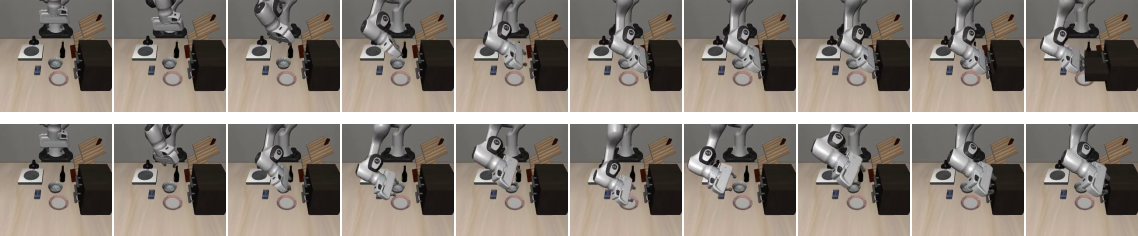
\includegraphics[width=0.99\textwidth]{figs/drawer_compare.png}
\caption{Filmstrips of two rollouts of the LIBERO \textsc{goal} task ``open the middle
drawer of the cabinet.'' \textbf{Top:} a successful rollout, collected with the co-trained
policy developed in this paper: the arm reaches the handle and pulls the drawer open.
\textbf{Bottom:} a failed rollout of the base policy: the arm hovers near the cabinet
without ever engaging the handle, until the episode times out.}
\label{fig:drawer}
\end{figure*}

The strongest current VLAs are no longer trained by imitation alone. With RECAP (RL with
Experience and Corrections via Advantage-conditioned Policies), Physical Intelligence showed
that a VLA can be improved past its imitation-learning baseline by training on its own
rollouts~\cite{b_recap}. The recipe has three ingredients. First, a \emph{critic} is trained
to estimate for every frame the \emph{value} $V(s_t)$, which is defined here as the expected
remaining time until task completion, normalized so that $-1$ corresponds to the start of an
episode and $0$ to completion. Second, every frame of the collected rollouts receives an
\emph{advantage}, computed as an $N$-step temporal-difference (TD) residual: the critic's
value $N$ frames later is compared with the value for the current frame, after accounting
for the $N$ steps of time that have passed. The advantage is therefore positive only when
the value rose by more than the elapsed time, that is, when the robot made more progress
over those $N$ frames than the critic expected. A clean grasp produces positive advantages, whereas a missed
grasp that must be retried produces negative ones. Third, the advantages are thresholded
into a binary \emph{advantage token}: every frame is labeled either positive or negative,
the token is prepended to the language instruction, and the policy is retrained with this
extra input. Because the token is dropped for a fraction of the training samples, the policy
learns three related predictors at once, namely one conditioned on good behavior, one
conditioned on bad behavior, and an unconditional one. In the original recipe the rollout
data additionally contains corrective human teleoperation, which inserts good behavior
exactly where the policy is weak. These results were demonstrated with $\pi^{*}_{0.6}$, a
large model that couples a $4$B-parameter Gemma~3 backbone with an $860$M-parameter action
expert.

The advantage token pays off at inference through classifier-free guidance
(CFG)~\cite{b_cfg}. To explain it, one more concept is needed. Like $\pi^{*}_{0.6}$, the
policies in this paper generate actions by flow matching~\cite{b_flow}: instead of
predicting an action chunk directly, the action expert learns a velocity field $v_\theta$
that transports a noise sample into an action chunk. Generating a chunk therefore means
solving an ordinary differential equation (ODE), which in practice is done with a small
fixed number of Euler integration steps, and each of these steps costs one forward pass
through the action expert. CFG steers this generation by replacing the learned field with
the \emph{guided velocity field}
\begin{equation*}
v^{\mathrm{cfg}}(x_t)=v_\theta(x_t)+w\,\big[v_\theta^{+}(x_t)-v_\theta(x_t)\big],
\end{equation*}
where $v_\theta$ is the unconditional prediction, $v_\theta^{+}$ is the prediction
conditioned on the positive advantage token, and $w$ is the guidance weight. The difference
$v_\theta^{+}-v_\theta$ points from typical behavior toward positively-labeled behavior.
Setting $w{=}0$ therefore recovers the unconditional policy, $w{=}1$ recovers the positive
conditional, and $w{>}1$ extrapolates past the positive mode, which pushes the generated
actions even further in the direction that the positive label rewards.

Our interest in this recipe comes from edge and mobile robotics, where such
post-training gains would matter most but where large models do not fit. The reference
inference stack for the $\pi$ model family lists more than $8$\,GB of GPU memory as the
inference requirement already for its released models that are smaller than
$\pi^{*}_{0.6}$~\cite{b_openpi}, and the documented example GPU, an RTX~4090, has a
$450$\,W board power rating. A battery-powered mobile robot offers a small fraction of that
budget. Our target onboard computer, an NVIDIA Jetson Orin NX $16$\,GB, operates within a
$10$--$25$\,W envelope, and its unified memory is shared with the operating system and the
rest of the robot's software stack~\cite{b_jetson}. The bfloat16 weights of
$\pi^{*}_{0.6}$ alone ($\approx 10$\,GB) would therefore leave roughly $6$\,GB for
everything else, such as cameras, inverse kinematics, and navigation, before accounting for
inference activations. SmolVLA~\cite{b_smolvla} was proposed as a compact alternative with
$450$M parameters and fits this class of hardware. At the moment, however, it only supports
imitation learning.

For this reason we study whether the RECAP recipe transfers to SmolVLA: if it does, the
gains of rollout post-training become available on exactly the robots that are restricted
to compact models. Our setting differs from the original one in three ways. First, the
policy is small, as motivated above. Second, all rollouts are collected fully autonomously,
because a deployed mobile robot rarely affords corrective teleoperation; instead, we mix
the original expert demonstrations back into fine-tuning as co-training batches, and we
will show that they take over the role that the human corrections play in RECAP. Third, we
pre-train the policy with knowledge insulation (KI)~\cite{b_ki}: the randomly initialized
action expert is trained while its gradients are blocked from entering the VLM backbone,
and the backbone is instead trained with an autoregressive loss on FAST-tokenized action
targets~\cite{b_fast}, which preserves its pretrained semantics. The original SmolVLA
recipe, in contrast, lets the flow-matching gradient train the backbone directly.

Rollout post-training is not the only way to improve a VLA past imitation. Other work
fine-tunes VLAs with online reinforcement learning (RL), which means the policy is updated
with policy gradients while it keeps interacting with the
environment~\cite{b_irevla,b_simplevlarl}, or aligns the policy with trajectory-level
preferences~\cite{b_grape}. We study the critic-relabeling recipe specifically because it
is the operationally simplest of these options: rollouts are collected offline, labeled by
a critic, and then reused as ordinary supervised training data, and therefore neither
reward shaping nor an online RL training loop is required.

A compact model alone does not make inference fast, because flow matching still integrates
the velocity field over ten Euler steps for every action chunk. For real-time control on
edge hardware we therefore add a final step, SnapFlow~\cite{b_snapflow} one-step
distillation. SnapFlow distills the multi-step expert into a one-step generator that is
conditioned on a target time: instead of following the velocity field step by step, the
distilled policy directly predicts the point that the full integration would reach, so a
single forward pass replaces the ten.

We run this pipeline on LIBERO and report the following:
\begin{itemize}
\item RECAP-style rollout post-training transfers to SmolVLA. The knowledge-insulation
recipe gains $5$--$11$ points per suite over a SmolVLA-style no-KI baseline. Rollout-only
training helps the short-horizon suites but degrades the long-horizon one, and adding
expert demonstrations to the fine-tuning mix counteracts the regression and gives the
strongest policies (Sec.~\ref{sec:main}).
\item An ablation of the advantage-labeling threshold (Sec.~\ref{sec:dose}). Setting it too
aggressively labels necessary actions as negative, which degrades the policy and makes CFG
counterproductive, whereas a relaxed threshold avoids this. Guidance itself pays off only
when the fine-tuning mix preserves distinct conditionals: it adds about one point for
rollout-only training and up to $6.6$ points after co-training.
\item Remaining failures concentrate on long-horizon tasks that chain two pick-and-place
subgoals, and co-training helps most on skills that are absent from the policy's own
rollouts (Sec.~\ref{sec:failure}).
\item One-step SnapFlow distillation of the best policy. Measured on a Jetson Orin Nano,
chunk generation drops from $922$ to $255$\,ms, while the success rate stays within two
average points of the ten-step policy. Baking CFG into the single step helps only where
guidance helps the original policy (Sec.~\ref{sec:snapflow}).
\end{itemize}
Taken together, the two building blocks complement each other: RECAP-style post-training
makes the compact policy better, and SnapFlow distillation makes it fast enough for the
hardware that the compact policy was chosen for in the first place.

\section{Method}
Our pipeline instantiates the RECAP recipe of the introduction with SmolVLA as the policy
and LIBERO as the benchmark. Fig.~\ref{fig:arch} gives an overview, and the following
subsections describe what each stage adds or changes relative to the recipe as described
so far.

\begin{figure}[t]
\centering
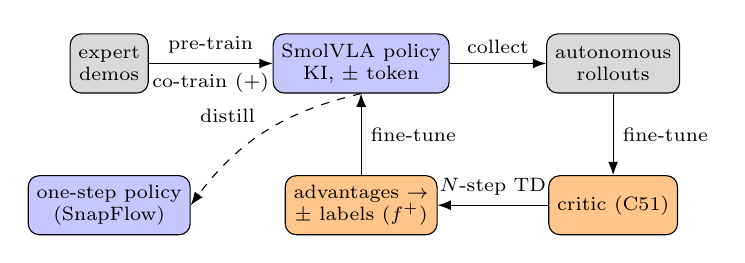
\begin{tikzpicture}[font=\scriptsize, >=Latex,
  box/.style={draw, rounded corners, align=center, inner sep=3pt, minimum height=7.5mm},
  data/.style={box, fill=gray!30},
  pol/.style={box, fill=blue!22},
  crit/.style={box, fill=orange!45}]
\node[pol]  (policy) at (0,0)       {SmolVLA policy\\KI, $\pm$ token};
\node[data] (demos)  at (-3.2,0)    {expert\\demos};
\node[data] (roll)   at (3.2,0)     {autonomous\\rollouts};
\node[crit] (critic) at (3.2,-1.8)  {critic (C51)};
\node[crit] (labels) at (0,-1.8)    {advantages $\to$\\$\pm$ labels (\pf)};
\node[pol]  (snap)   at (-3.2,-1.8) {one-step policy\\(SnapFlow)};
\draw[->] (demos) -- node[above]{pre-train} node[below]{co-train ($+$)} (policy);
\draw[->] (policy) -- node[above]{collect} (roll);
\draw[->] (roll) -- node[right]{fine-tune} (critic);
\draw[->] (critic) -- node[above]{$N$-step TD} (labels);
\draw[->] (labels) -- node[right]{fine-tune} (policy);
\draw[->, dashed] (policy.south) to[bend right=20] node[above left]{distill} (snap.east);
\end{tikzpicture}
\caption{Pipeline overview. Gray: data; blue: policies; orange: critic and labeling.
Expert demonstrations pre-train the advantage-conditioned policy and re-enter fine-tuning
as always-positive co-training batches. The policy collects autonomous rollouts, on which
the critic (itself first trained on the demonstrations) is fine-tuned; $N$-step advantages
are thresholded at positive fraction \pf{} into the $\pm$ tokens that condition
fine-tuning and enable CFG at inference. SnapFlow distills the fine-tuned ten-step policy
into a single step for edge deployment.}
\label{fig:arch}
\end{figure}

\subsection{Critic and advantage-conditioned pre-training}\label{sec:pretrain}
Before training the policy, a distributional (C51)~\cite{b_c51} critic is trained on the
LIBERO expert dataset to predict the remaining time to episode completion as a categorical
distribution over $201$ bins spanning the normalized range $[-1,0]$; its expectation is the
value $V(s_t)$. For convenience the critic reuses the policy's architecture and consumes
the same observations. Its VLM backbone is truncated to eight layers, and the action head
is replaced by the categorical value head. Fig.~\ref{fig:critic} shows the critic's value
estimate over an expert episode: the value rises steadily as the robot makes progress and
temporarily drops back when progress stalls, for example after a missed grasp. This
within-trajectory structure is what makes per-frame advantages informative.

\begin{figure}[t]
\centering
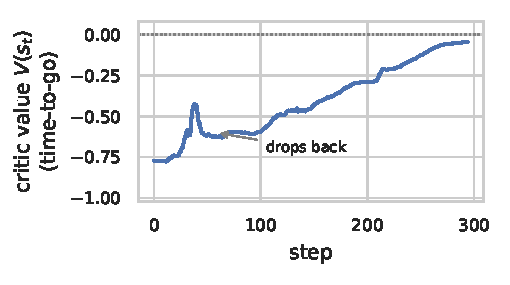
\includegraphics[width=\columnwidth]{figs/fig_critic.pdf}
\caption{Value estimate $V(s_t)$ of the demonstration-trained critic over one expert
episode. The value is the expected normalized time-to-completion, so $-1$ means the start
of the episode and $0$ means the task is done; it is a prediction of the critic, not an
environment reward.}
\label{fig:critic}
\end{figure}

The base policy, denoted $\pi_{\text{base}}$ from here on, is then pre-trained for $250$k
steps on the same expert dataset with KI \emph{and advantage conditioning already in
place}: per-frame advantages from the demonstration-trained critic are thresholded per task
into positive/negative tokens that are prepended to the language prefix. The token is
dropped with probability $0.3$, so that an unconditional predictor is learned alongside the
two conditionals.

\subsection{Rollout collection and critic fine-tuning}
$\pi_{\text{base}}$ collects rollouts on the target suites, which yields $107{,}410$ frames
over $600$ episodes with a success rate of $64.3\%$. All rollouts are collected
autonomously, so no human teleoperation corrections or interventions are used. The critic
is then fine-tuned on this rollout data with a pessimistic target for failed episodes: a
large constant is added to their remaining time to completion, which after normalization
clamps their return target to the bottom of the value support ($-1$). This step is
necessary because the demonstration-trained critic, having seen only successful
demonstrations, was over-optimistic on failed rollouts and assigned them values close to
those of successes. After fine-tuning, per-frame advantages are computed as $N$-step TD
residuals with $N{=}50$. Through the pessimistic returns, frames of failed episodes receive
strongly negative advantages. These advantages provide the thresholds and labels for the
subsequent policy fine-tuning.

\subsection{Advantage labeling}
The labeling is controlled by a single parameter, the target positive fraction \pf{}: the
letter $f$ stands for the fraction of frames that receive the positive-advantage label,
and the superscript $+$ for that positive label. For each task, a threshold
$\varepsilon_\ell$ is set to the $100(1-\pf)$th percentile of the advantage distribution
over that task's \emph{successful} frames, so that a fraction \pf{} of them keeps the
positive label. A frame is labeled positive if its advantage exceeds $\varepsilon_\ell$ and
negative otherwise. A small \pf{} therefore labels frames negative aggressively, while
$\pf{}$ close to $1$ reserves the negative label for the worst frames. We use $\pf{=}0.8$
as the default and ablate lower values in Sec.~\ref{sec:dose}. We also evaluate an
\emph{outcome-only} scheme that bypasses the critic entirely: every frame of a successful
episode is positive, and every frame of a failed episode is negative.

\subsection{Advantage-conditioned fine-tuning and CFG}
The policy is fine-tuned from $\pi_{\text{base}}$ on the rollout data, with the rollout
labels supplying the positive/negative token that pre-training established. The same $0.3$
token dropout keeps the unconditional predictor required for CFG intact. At inference the
expert integrates the guided velocity field of the introduction in ten fixed Euler steps,
and we sweep the guidance weight $w\in\{0,0.5,1,1.5,2\}$.

\subsection{Expert co-training}
We also co-train on the expert demonstrations: at each training step the batch is drawn
from the demonstrations with probability $0.5$, and all demonstration frames are labeled
positive. This supplies known-good behavior for the positive conditional, including skills
that may be absent from the policy's own rollouts. In addition it acts as replay against
forgetting behavior that was learned in pre-training but is not exercised in the rollout
data.

\subsection{SnapFlow distillation}
Given the best fine-tuned policy, SnapFlow distills its ten-step expert into a single-step
generator. The distilled expert is conditioned on a target time and trained to jump
directly to the action chunk that the teacher's full ten-step Euler integration would
produce, so that one forward pass replaces the iterative integration at inference.
Training combines a flow-matching term anchored on the training data with a distillation
term that matches the one-step jump to the teacher's multi-step result; in the default
progressive self-distillation setup, the training model itself supplies the teacher
targets. The distilled policy is initialized from the original one, so distillation starts
from the original policy's behavior.

\section{Experimental Setup}\label{sec:setup}
\textbf{Benchmark.} We evaluate on the three LIBERO suites introduced above:
\textsc{spatial}, \textsc{goal}, and \textsc{long} (LIBERO-10). We do not use the fourth
suite, \textsc{object}, because every policy trained in our setting, including the base,
runs its episodes to timeout without completing the task. A control experiment locates the
cause: re-running the base pre-training unchanged except for photometric image augmentation
lifts \textsc{object} from $0\%$ to $53.6\%$ while staying within evaluation noise on the
three reported suites (average $63.5$ vs.\ $62.9$). The failure is thus a visual domain gap
that augmentation closes, and neither corrupted demonstrations nor a property of the
methods. Since all configurations compared here are trained without augmentation, the suite
affects them identically and therefore cannot separate them.

\textbf{Protocol.} Every reported number is the success rate in percent over $50$ episodes
per task, which gives $n{=}500$ episodes per suite, taken at the method's best guidance
weight. Suite averages are the unweighted mean of the three suite values. All
advantage-conditioned methods are swept identically over $w\in\{0,0.5,1,1.5,2\}$. The
no-KI baseline, whose constant conditioning admits no meaningful guidance, is evaluated at
its single operating point $w{=}1$.

\textbf{Models.} All policies use the SmolVLA architecture ($450$M parameters, a
$16$-layer VLM backbone with a flow-matching action expert), and the critic shares this
architecture with the backbone truncated to $8$ layers. The base policy is pre-trained for
$250$k steps on the expert demonstrations with KI, FAST co-training, and advantage
conditioning; all fine-tuning runs take $20$k steps. The no-KI baseline mirrors the
original SmolVLA objective: flow-matching gradients from the action expert train the VLM
directly (no insulation), replacing the FAST AR co-training as the VLM's training signal,
and the advantage token is held constant (every training frame positive, no token dropout),
which reduces the conditioning to an inert extra token. All remaining settings (optimizer,
schedule, action chunking, data, $250$k steps) are shared with the base. The comparison
therefore measures the KI training recipe as a whole rather than gradient insulation in
isolation; both models are trained under our harness settings rather than the lerobot
SmolVLA presets.

\textbf{Comparability with published SmolVLA results.} The released SmolVLA is pre-trained
on a large corpus of community robot datasets; reproducing this was not feasible within our
compute budget, so every model here is trained on the LIBERO expert demonstrations
(\texttt{HuggingFaceVLA/libero}) alone, and our absolute numbers are not directly
comparable to published ones. Evaluated under our protocol, the released LIBERO fine-tune
(\texttt{HuggingFaceVLA/smolvla\_libero}) scores close to our no-KI baseline, which is
therefore a faithful stand-in for the original recipe in our setting. Training and
evaluation hardware and run times are listed in Appendix~\ref{app:compute}.

\section{Results}
\subsection{Rollout post-training transfers to SmolVLA}\label{sec:main}
Table~\ref{tab:main} reports the success rate of each configuration on each suite at its
best guidance weight. The KI training recipe is the largest single effect: the KI base
beats the no-KI baseline by $5$ to $11$ points per suite ($+6.2$ on \textsc{spatial},
$+5.2$ on \textsc{goal}, and $+11.4$ on \textsc{long}). Training on critic-labeled rollout
data alone ($\pf{=}0.8$) improves the KI base on \textsc{spatial} ($+6.6$) and
\textsc{goal} ($+4.2$), but it \emph{degrades} \textsc{long} ($35.8\%$ vs.\ $41.6\%$).
Mixing expert demonstrations into fine-tuning lifts every suite over rollout-only training
and yields the two best configurations, with $68.1\%$ and $67.8\%$ average success
compared to $62.9\%$ for the base. The \textsc{long} regression, however, is only
mitigated at $\pf{=}0.8$ ($38.2\%$, still below the base's $41.6\%$) and fully repaired at
$\pf{=}0.4$ ($43.8\%$). At a suite-level standard error of about $\pm2$ points these
threshold effects sit at the edge of resolution, and we return to them in
Sec.~\ref{sec:discussion}.

\begin{table}[t]
\caption{Main comparison on the three LIBERO suites. Each cell is the success rate in
percent ($n{=}500$ episodes per suite) at the method's best guidance weight; avg is the
unweighted mean of the three suites, and ms/chunk is the latency for generating one
$20$-action chunk.}
\label{tab:main}
\begin{center}
\begin{tabular}{lccccc}
\toprule
method & spatial & goal & long & avg & ms/chunk \\
\midrule
SmolVLA, no KI            & 65.0 & 70.6 & 30.2 & 55.3 & -- \\
SmolVLA $+$KI (base)      & 71.2 & 75.8 & 41.6 & 62.9 & -- \\
$+$rollout data (\pf{}=0.8) & 77.8 & 80.0 & 35.8 & 64.5 & -- \\
$+$co-training (\pf{}=0.4)   & 75.4 & 84.2 & \textbf{43.8} & 67.8 & -- \\
$+$co-training (\pf{}=0.8)   & \textbf{80.0} & \textbf{86.2} & 38.2 & \textbf{68.1} & 922 \\
  $+$SnapFlow distillation     & 74.2 & 84.2 & 40.0 & 66.1 & \textbf{255} \\
\midrule
outcome-only              & 72.8 & 81.8 & 40.0 & 64.9 & -- \\
\bottomrule
\end{tabular}
\end{center}
{\footnotesize $+$ marks additions to the pipeline: rollout fine-tuning on the KI base,
co-training at two labeling thresholds, and one-step distillation of the $\pf{=}0.8$
policy (Sec.~\ref{sec:snapflow}). ``outcome-only'' labels frames by episode outcome only.
Latency: one $20$-action chunk, Jetson Orin Nano, bfloat16; measured configurations only.}
\end{table}

\subsection{Ablation: the advantage-labeling threshold}\label{sec:dose}
The threshold controls how many frames are labeled negative, and Table~\ref{tab:labels}
shows the resulting label composition of the rollout data for three values of \pf{}. At low
\pf{} ($0.3$ and $0.4$), between $26\%$ and $31\%$ of all frames are frames \emph{inside
successful trajectories} that nevertheless receive the negative label. These are to a large
extent the approach and transport motions a task requires, and the policy is consequently
trained to treat necessary actions as behavior to avoid.

\begin{table}[t]
\caption{Label composition of the rollout data under each labeling scheme, in percent of
all frames.}
\label{tab:labels}
\begin{center}
\begin{tabular}{lcccc}
\toprule
scheme & pos\% & neg\% & pos{:}fail & neg{:}succ \\
\midrule
\pf{}=0.3 & 15.0 & 85.0 & 1.7 & 30.9 \\
\pf{}=0.4 & 20.7 & 79.3 & 3.0 & 26.5 \\
\pf{}=0.8 & 51.5 & 48.5 & 16.2 & 8.9 \\
outcome-only & 44.2 & 55.8 & 0.0 & 0.0 \\
\bottomrule
\end{tabular}
\end{center}
{\footnotesize All $107{,}410$ rollout frames, failures included. ``pos{:}fail'': frames in
failed episodes labeled positive; ``neg{:}succ'': frames in successful episodes labeled
negative (percent of all frames).}
\end{table}

Table~\ref{tab:dose} shows the consequences on the \textsc{spatial} suite as a sweep over
the guidance weight. At $\pf{=}0.3$ the entire sweep sits below the base ($67.0\%$ at
$w{=}0$ vs.\ $71.2\%$). At $\pf{=}0.4$ the unguided policy still edges out the base
($72.8\%$), but guidance erodes it steadily down to $65.4\%$ at $w{=}2$. This is the
failure mode that the guided velocity field predicts for a mislabeled dataset: because many
necessary motions were labeled negative, the positive conditional $v_\theta^{+}$ no longer
contains them, the difference $v_\theta^{+}\!-\!v_\theta$ therefore points \emph{away} from
those motions, and increasing $w$ pushes the policy ever further along exactly this
direction. At $\pf{=}0.8$ the negative label is reserved for genuinely low-advantage
behavior, which mostly comes from failed episodes. The policy then improves over the base,
and moderate guidance helps. For this reason we use $\pf{=}0.8$ throughout.

\begin{table}[t]
\caption{Guidance-weight sweep on \textsc{spatial}. Each cell is the success rate in
percent at the given guidance weight $w$.}
\label{tab:dose}
\begin{center}
\begin{tabular}{lcccccc}
\toprule
scheme & pos\% & $w{=}0$ & $0.5$ & $1$ & $1.5$ & $2$ \\
\midrule
\pf{}=0.3 & 15 & 67.0 & 66.6 & 66.0 & 67.4 & 63.0 \\
\pf{}=0.4 & 21 & 72.8 & 70.8 & 70.4 & 67.4 & 65.4 \\
\pf{}=0.8 & 52 & 76.8 & \textbf{77.8} & 75.4 & 72.6 & 72.4 \\
\bottomrule
\end{tabular}
\end{center}
\end{table}

Even in this best case, guidance itself is a minor contributor for the rollout-only
policy: it adds $+1.0$ points on \textsc{spatial} ($76.8\%$ at $w{=}0$ vs.\ $77.8\%$ at
$w{=}0.5$), while nearly all of the gain over the base is already present at $w{=}0$
($76.8\%$ vs.\ $71.2\%$). In other words, the gain comes from the advantage-conditioned
fine-tuning on labeled rollouts rather than from steering at inference. The picture
changes once demonstrations are co-trained: the co-trained $\pf{=}0.8$ policy gains
$+6.6$ points on \textsc{spatial} from guidance ($73.4\%$ at $w{=}0$ to $80.0\%$ at
$w{=}1.5$) and $+2.4$ points on \textsc{goal}. A possible reading, developed in
Sec.~\ref{sec:discussion}, is that the demonstration batches keep the conditional and
unconditional modes separated, so that inference-time steering has a direction to amplify.

The negative-token probe points the same way: forcing the \emph{negative} token at
inference costs only $1$--$2$ points relative to the positive token on \textsc{spatial}
and \textsc{goal} ($w{=}1$). For the $\pf{=}0.3$ policy the probe finds no usable
separation at all (negative $66.4\%$ vs.\ positive $66.0\%$ on \textsc{spatial}; on
\textsc{goal} the negative token even scores higher, $76.4\%$ vs.\ $73.6\%$). With a third
of the successful frames labeled negative, the token never carried a good/bad distinction.
The positive, negative, and unconditional predictions are compressed into a narrow band,
and as a result the $v_\theta^{+}\!-\!v_\theta$ difference that guidance amplifies is
small. On \textsc{long} the separation is similarly modest: forcing the negative token
costs $1.0$ point for the $\pf{=}0.8$ policy ($34.8\%$ vs.\ $35.8\%$) and $3.8$ points for
$\pf{=}0.4$ ($29.4\%$ vs.\ $33.2\%$). Part of this may be limited headroom over the base
policy, and part may be a capacity effect, to which we return in
Sec.~\ref{sec:discussion}.

\subsection{Where the policies still fail}\label{sec:failure}
Per-task results at $50$ trials carry substantial binomial noise ($\approx\pm14\%$ at
$95\%$ confidence), so we restrict the discussion to patterns that are consistent across
methods and clearly outside that noise.

The dominant remaining failure mode is the long-horizon tasks, which chain two
pick-and-place subgoals in one instruction. All methods stay below $\sim40\%$ on the same
subset of \textsc{long} tasks of this type, and on the hardest of them (``put both the
alphabet soup and the cream cheese box in the basket'') every method stays below $16\%$.
The policy typically places the first object and then fails to sequence the second before
timeout. Single-subgoal \textsc{long} tasks, in contrast, reach $70$--$80\%$, which is
comparable to the other suites. The low \textsc{long} averages therefore reflect error
compounding across subgoals rather than a deficiency of any particular post-training
method.

Second, co-training helps most where the rollout data cannot: on skills the base policy
never executes successfully, its rollouts contain no positive examples, so rollout
post-training has nothing to reinforce. Drawer manipulation is the clearest case. The base
policy's rollouts contain no successful drawer opening, and only the co-trained policy
acquires the skill (Fig.~\ref{fig:drawer}). Rollout data can only sharpen behavior the
policy already shows; skills it lacks entirely have to come from the demonstrations.

\subsection{Critic granularity: outcome-only labels}
The outcome-only scheme tests whether the critic's within-trajectory granularity matters,
or whether a plain success/failure label suffices. The answer is mixed. Outcome-only
reaches $72.8\%$ on \textsc{spatial}, five points below the critic-labeled $\pf{=}0.8$
policy ($77.8\%$), but $81.8\%$ on \textsc{goal}, slightly ahead of it ($80.0\%$), and
$40.0\%$ on \textsc{long}, also ahead ($35.8\%$). On average the two schemes are
indistinguishable ($64.9\%$ vs.\ $64.5\%$): the critic's within-trajectory granularity is
not required to benefit from rollout data on these suites, although the best overall
configuration (co-training) does use it. We have not combined outcome-only labels with
co-training; that run would isolate the critic's contribution to the best configuration
and is left for future work.

\subsection{SnapFlow: one-step inference}\label{sec:snapflow}
We distill the co-trained $\pf{=}0.8$ policy, which is the strongest configuration on the
two short-horizon suites and on average. On edge robots, long-horizon tasks are often
decomposed by a higher-level planner, so short-horizon competence is the relevant
operating regime.

\textbf{Distillation quality.} The distilled policy is trained on the same data mixture
the original was fine-tuned on, that is, critic-labeled rollout data with demonstration
batches at ratio $0.5$. The rollout frames keep their critic labels, because forcing them
all positive would make the flow-matching term imitate advantage-negative rollout actions
under the positive token. The distilled policy reaches $74.2\%$/$84.2\%$/$40.0\%$
(Table~\ref{tab:distill}), which is within $2.0$ average points of the ten-step original
and matches it on \textsc{long}. Distilling longer hurts: in a preliminary variant without
the demonstration mix, extending distillation from $15$k to $120$k steps kept lowering the
distillation loss ($0.106$ to $0.047$) while average closed-loop success dropped by about
ten points. This is a form of over-distillation, and for this reason all distilled
policies are trained for $15$k steps. Finally, following guided-diffusion
distillation~\cite{b_cfgdistill}, we try baking the guidance into the distilled policy by
distilling the CFG-blended field of the original at $w{=}1.5$, so that a single unguided
pass reproduces guided behavior. With the training model supplying its own distillation
targets (progressive self-distillation) this fails ($57.3\%$ average): the data-anchored
flow-matching term pulls the distilled policy toward the unguided field, and the blend's
unconditional branch, trained by no loss term, drifts. A \emph{frozen} copy of the
original supplying both loss terms recovers the mechanism where guidance helps the
original most: on \textsc{spatial} the guidance-baked policy reaches $76.8\%$ in a single
pass, within $3.2$ points of the guided original, but it loses on \textsc{goal} and
especially on \textsc{long}, where one-step integration of the extrapolated field appears
to overshoot. Guidance baking is therefore worthwhile only where the original demonstrably
profits from $w{>}1$. The plain distilled policy remains our deployed configuration,
averaging $64.5$--$64.7\%$ at its single-pass operating points ($w\in\{0,1\}$; other
weights double the action expert's batch at inference).

\begin{table}[t]
\caption{SnapFlow distillation ablation. Each cell is the success rate in percent; avg is
the mean of the three suites.}
\label{tab:distill}
\begin{center}
\begin{tabular}{lcccc}
\toprule
policy & spatial & goal & long & avg \\
\midrule
distilled policy                  & 74.2 & \textbf{84.2} & \textbf{40.0} & \textbf{66.1} \\
$+$guidance baked, self-distilled & 67.0 & 72.4 & 32.6 & 57.3 \\
$+$guidance baked, frozen original & \textbf{76.8} & 75.2 & 25.2 & 59.1 \\
\midrule
original ($10$-step FM)           & 80.0 & 86.2 & 38.2 & 68.1 \\
\bottomrule
\end{tabular}
\end{center}
{\footnotesize All distilled policies are trained for $15$k steps from the co-trained
$\pf{=}0.8$ policy on its fine-tuning mixture: critic-labeled rollouts with demonstration
batches at ratio $0.5$.}
\end{table}

\textbf{Latency.} We measure inference on an NVIDIA Jetson Orin Nano ($8$\,GB unified
memory), running the policy in bfloat16 (setup in Appendix~\ref{app:compute}). Generating
one $20$-action chunk takes $922\pm1$\,ms with the ten-step flow-matching integration and
$255\pm1$\,ms with SnapFlow's single step. This is a $3.6\times$ speed-up, and it raises
the re-planning rate from $1.1$ to $3.9$ chunks per second ($12.7$\,ms per action
amortized over the chunk). Our target device, the Jetson Orin NX ($16$\,GB), reproduces
these numbers within $8\%$ (Appendix~\ref{app:compute}). The remaining $255$\,ms is
dominated by the vision-language prefix, which both variants share.

\section{Discussion and Limitations}\label{sec:discussion}
Our results show that the RECAP recipe can also improve a compact VLA, with two practical
qualifications. First, the advantage-labeling threshold should be set permissively, which
in our notation means \pf{} close to $1$: our best setting keeps $80\%$ of the successful
frames positive ($\pf{=}0.8$), whereas the aggressive settings ($\pf{=}0.3$ and $0.4$)
labeled necessary actions negative and the policy partially unlearned them. Second,
rollout-only fine-tuning is not uniformly safe: it degraded the long-horizon suite, and
rollouts can only reinforce behavior the policy already exhibits. Mixing demonstration
batches into fine-tuning addressed both issues in our experiments.

The suite-level pattern suggests that rollout post-training amplifies the quality of the
rollouts it is fed. On \textsc{spatial} and \textsc{goal}, where roughly three quarters of
the base policy's episodes succeed, the labeled rollouts contain plenty of good behavior
to reinforce, and rollout-only training helps. On \textsc{long}, where most rollouts fail,
even the positively labeled frames come from largely mediocre behavior; fine-tuning on
them amounts to learning from a weak teacher, and the policy falls below its starting
point. Notably, RECAP's corrective teleoperation inserts good behavior exactly where the
policy lacks it, and in our autonomous setting the co-trained demonstrations take over
that role. One possible explanation for why co-training matters more here than in RECAP is
model capacity: a compact policy may not have the capacity to retain its pre-training
behavior through rollout-only fine-tuning, so the demonstration batches act as explicit
replay against forgetting. The same limit may explain the guidance results: after
rollout-only fine-tuning the positive, negative, and unconditional predictions are
compressed into a narrow band and CFG has little to amplify, whereas the co-trained
policy, whose demonstration replay would preserve the separated modes, is the one policy
that gains substantially from guidance. Our experiments are consistent with this capacity
view but do not isolate it. The co-training runs also show that the long-horizon
regression is not specific to rollout-only training: co-training at $\pf{=}0.8$ reduces it
without removing it, while the $\pf{=}0.4$ co-trained run clears it, so on \textsc{long}
the labeling threshold may matter as much as the data mix, though these differences sit at
the edge of the $\pm2$-point resolution. One hypothesis is the following: most
\textsc{long} rollout episodes fail, so at $\pf{=}0.4$ almost no failure frames carry the
positive token ($3.0\%$ of all frames vs.\ $16.2\%$ at $\pf{=}0.8$) and the positive
conditional is learned almost entirely from the co-trained demonstrations, whereas at
$\pf{=}0.8$ it also absorbs behavior from failed rollouts, on exactly the suite where the
rollouts are weakest. The usual cost of the aggressive threshold is covered by the
demonstrations, which supply the necessary actions it strips from the rollout positives.

Limitations: all results are in simulation on LIBERO with a single training seed per
configuration, and per-task numbers at $50$ trials are noisy, so we draw conclusions only
from suite-level aggregates. Reporting the maximum over a five-point guidance sweep
carries an optimistic bias of one to two points, which is on the order of the suite-level
standard error. Every advantage-conditioned method receives the identical sweep, so
comparisons among them are unaffected; absolute numbers are slightly flattered, and the
no-KI baseline, which has a single operating point, lacks this benefit. We tested positive
fractions $0.3$, $0.4$, and $0.8$ only. Latency was measured on-device but not in
closed-loop control.

\section{Conclusion}
Critic-guided rollout post-training transfers from large VLAs to SmolVLA: pre-training
with knowledge insulation improves over a SmolVLA-style no-KI baseline, and fine-tuning on
critic-labeled rollouts mixed with expert demonstrations yields the best policy on each
suite, although no single labeling threshold wins all three. One-step SnapFlow
distillation preserves this within two average points while cutting on-device latency
$3.6\times$. Rollout-based improvement of VLA policies is therefore a practical option for
the compact models that edge and mobile robots can run.

\appendices
\section{Training and evaluation infrastructure}
\label{app:compute}
All training and evaluation ran on the FHNW high-performance computing infrastructure.
Pre-training ($250$k steps) takes $\approx18$~h on two NVIDIA H200 GPUs, and each
fine-tuning run takes $20$k steps ($\approx90$~min on one H200). Evaluation is
simulation-bound rather than GPU-bound: a full $n{=}500$ suite evaluation takes
$2.5$--$6$~h on an H200 and only $1.5$--$3.2\times$ longer on much smaller GPUs
(RTX~A4500, RTX~2080). For this reason evaluations ran on the smaller GPUs, reserving the
H200 nodes for training.

\textbf{Edge latency measurement.} The latencies reported in the main text were measured
on an NVIDIA Jetson Orin Nano ($8$\,GB unified memory) running JetPack~6 and
PyTorch~2.11. The policy is the deployed architecture and runs in bfloat16 under autocast
with batch size~$1$, two $256{\times}256$ cameras, and $48$ language tokens. Each number
is the mean over $30$ timed chunk generations after $8$ warm-up iterations, and the
standard deviation is about $1$\,ms. Table~\ref{tab:edge} repeats the measurement on a
Jetson Orin NX ($16$\,GB), where the bfloat16 numbers reproduce within $8\%$. In float32,
which would exceed the Orin Nano's memory, the SnapFlow latency more than doubles and its
speed-up shrinks to $2\times$, because the shared vision-language prefix then dominates
the runtime. Bfloat16 is therefore the practical deployment dtype.

\begin{table}[t]
\caption{Action-chunk latency (ms) on edge devices}
\label{tab:edge}
\begin{center}
\begin{tabular}{llccc}
\toprule
device & dtype & FM ($10$ steps) & SnapFlow & speed-up \\
\midrule
Orin Nano $8$\,GB & bf16 & $922$ & $255$ & $3.6\times$ \\
Orin NX $16$\,GB  & bf16 & $850$ & $240$ & $3.5\times$ \\
Orin NX $16$\,GB  & fp32 & $1143$ & $575$ & $2.0\times$ \\
\bottomrule
\end{tabular}
\end{center}
\end{table}

\section*{Acknowledgment}
Training and evaluation were carried out on the FHNW high-performance computing
infrastructure, which made these experiments possible.

\begin{thebibliography}{00}
\bibitem{b_libero} B. Liu et al., ``LIBERO: Benchmarking knowledge transfer for lifelong
robot learning,'' arXiv:2306.03310, 2023.
\bibitem{b_recap} A. Amin et al., ``$\pi^{*}_{0.6}$: a VLA that
learns from experience,'' arXiv:2511.14759, 2025.
\bibitem{b_cfg} J. Ho and T. Salimans, ``Classifier-free diffusion guidance,'' in
\emph{NeurIPS Workshop on Deep Generative Models and Downstream Applications}, 2021.
\bibitem{b_flow} Y. Lipman et al., ``Flow matching
for generative modeling,'' in \emph{Proc.\ ICLR}, 2023.
\bibitem{b_openpi} Physical Intelligence, ``openpi: Open-source robot foundation models,''
\url{https://github.com/Physical-Intelligence/openpi}, accessed July 2026.
\bibitem{b_jetson} NVIDIA, ``Jetson modules: Jetson Orin Nano series,''
\url{https://developer.nvidia.com/embedded/jetson-modules}, accessed July 2026.
\bibitem{b_smolvla} M. Shukor et al., ``SmolVLA: A vision-language-action model for
affordable and efficient robotics,'' arXiv:2506.01844, 2025.
\bibitem{b_ki} D. Driess et al., ``Knowledge insulating vision-language-action models: Train
fast, run fast, generalize better,'' arXiv:2505.23705, 2025.
\bibitem{b_fast} K. Pertsch et al., ``FAST: Efficient action tokenization for
vision-language-action models,'' arXiv:2501.09747, 2025.
\bibitem{b_irevla} Y. Guo et al., ``Improving vision-language-action model with online
reinforcement learning,'' arXiv:2501.16664, 2025.
\bibitem{b_simplevlarl} H. Li et al., ``SimpleVLA-RL: Scaling VLA training via reinforcement
learning,'' arXiv:2509.09674, 2025.
\bibitem{b_grape} Z. Zhang et al., ``GRAPE: Generalizing robot policy via preference
alignment,'' arXiv:2411.19309, 2024.
\bibitem{b_snapflow} W. Luan et al., ``SnapFlow:
One-step action generation for flow-matching VLAs via progressive self-distillation,''
arXiv:2604.05656, 2026.
\bibitem{b_c51} M. G. Bellemare, W. Dabney, and R. Munos, ``A distributional perspective on
reinforcement learning,'' in \emph{Proc.\ ICML}, 2017.
\bibitem{b_cfgdistill} C. Meng et al., ``On distillation of guided diffusion models,'' in
\emph{Proc.\ CVPR}, 2023.
\end{thebibliography}

\end{document}
